\chapter{Introduction}

%The introduction chapter contains a brief introduction for the
%application that explains what it does and where to report
%problems. Basically a long version of the abstract.  Don't include a
%revision history. (see installation appendix comment)

\label{sec-scidavis-intro}
\section{What is \SciDaVis?}

\SciDaVis{} stands for {\em Sci}entific {\em D}ata {\em A}nalysis and
         {\em Vis}ualization. It is a free cross-platform program for
         two- and three-dimensional graphical presentation of data
         sets and for data analysis. The plots can be produced from
         data sets stored in \htmlref{tables}{sec-intro-table}, in
         \htmlref{matrix}{sec-intro-matrix} or from analytical
         functions.
         
The \SciDaVis{} project started as a fork of QtiPlot with the aim of
introducing some changes in design as well as project structure. The
QtiPlot development was initiated in 2004 by Ion Vasilief. He was the
only programmer until May 2006 when Knut Franke and Tilman Hoener zu
Siederdissen joined the project. Not much later, Roger Gadiou
officially joined as the main documentation writer. In June 2007,
insuperable disagreements among the developers lead to the fork and
the creation of the \SciDaVis{} project by Knut and Tilman, soon
followed by Roger. In November 2012, after approximately two years of
inactivity in the project, Russell Standish assumed the development of
\SciDaVis. The project is hosted partially at
\htmladdnormallink{Sourceforge}{https://sourceforge.net/projects/scidavis/}
(download files, the bug tracker, forums, mailing lists, etc.), but
its source code development was moved from the \SciDaVis{} subversion
repository to
\htmladdnormallink{Github}{https://github.com/highperformancecoder/scidavis} in
June 2015.

\SciDaVis{} aims to be a tool for analysis and graphical
representation of data, allowing powerfull mathematical treatment and
visualization of scientific data while keeping a user-friendly
graphical user interface. Another keypoint for the \SciDaVis{} project
is to be a multi-system software, it should work on Windows, Linux,
and OS-X systems.

\SciDaVis{} is a dynamic tool, the plots created from data sets and
the spreadsheets owing the data are interconected. When the
spreadsheets are modified, all the objects in the depending plots
(curves, axes scales, legends) are automatically updated. For example,
deleting a spreadsheet or only some columns will automatically remove
all the corresponding curves from the depending plots.

All settings of a complete set of tables, matrix and plots can be
saved in project files, having the extention ``.sciprj". These project
files may be opened using the \htmlref{command line}{specify-a-file},
using the \htmlref{File menu}{file-menu-lnk}, or by using the
\htmladdimg{icons/fileopen.png} icon from the \htmlref{File
  toolbar}{file-toolbar-lnk}.

The plots can be exported to several graphic formats such as JPEG or
PNG and inserted as images in documents or presentations.

Data analysis operations (integration, interpolation, FFT, curve
fitting, etc) can be performed on the curves in a 2D plot via the
\htmlref{Analysis-plots menu}{analysis-plots-menu-lnk}. The results of
all these operations are also stored in the project files. They can be
visualized at any moment using the \htmlref{Results Log command}{results-log-lnk} and can be
deleted from the project file via the \htmlref{Clear Log Information command}{clear-log-information-lnk}.

When the application is launched, a new project file is created
consisting of a grey main window (the workspace) which contains an
empty table. In order to be operational, this workspace must be
populated with tables storing data sets, either by creating empty
tables first (\htmlref{New $\rightarrow$ New Table
  command}{new-table-lnk}) and then filling them with data, or by
importing ASCII files (\htmlref{Import ASCII
  command}{import-ascii-lnk}), which automatically creates new tables.

The user can easily navigate through the objects of a project file
using the \htmlref{Project Explorer command}{project-explorer-lnk} or
the \htmlref{Windows menu}{windows-menu-lnk}. The project explorer
also allows the user to perform various operations on the windows
(tables and plots) in the workspace: hiding, minimazing, closing,
renaming, printing, etc.

%************************************************************************
%
%			Command line parameters
%
%************************************************************************
\section{Command Line Parameters}\label{command-line-options}

\subsection{Specify a File}\label{specify-a-file}
\index{Command line parameters!Specify a File}

When starting \SciDaVis{} from the command prompt, you can supply the name of a project file:

\begin{verbatim}
scidavis file_name.sciprj
\end{verbatim}

Other file format are also accepted: {\em .opj, .ogm, .ogw, .ogg} for
Origin projects, and {\em .qti, qti.gz} for Qtiplot projects.

The name can also refer to an ASCII file:

\begin{verbatim}
scidavis ASCII_file_name
\end{verbatim}

In this latter case a new ``untitled" project will be created,
containing a spreadsheet with the ASCII data in the file and a 2D plot
of all columns as a function of the first column in the file. You must
take care of the format of the ASCII file because it will be read with
the current parameters of the \htmlref{Import ASCII
  command}{import-ascii-lnk} dialog. The default values are:

\begin{itemize}
  \item the default field separator is ; but it can be changed in the
    \htmlref{Preferences command}{preferences-lnk} dialog,
  \item all lines are read,
  \item the first line is used to name the columns,
  \item the spaces at the end of the lines are not removed,
  \item the spaces are not simplified.
\end{itemize}

\subsection{Command Line Options}\label{scidavis-options}
\index{Command line parameters!Options}

Valid options are:
\begin{itemize}
\item \verb+-a+ or \verb+--about+: show about dialog and exit
\item \verb+-h+ or \verb+--help+: show command line options
\item \verb+-l=XX+ or \verb+--lang=XX+: start \SciDaVis; in language XX (`en', `fr', `de', \ldots)
\item \verb+-m+ or \verb+--manual+: show \SciDaVis{} manual in a standalone window
\item \verb+-v+ or \verb+--version+: print \SciDaVis{} version and release date
\item \verb+-x+ or \verb+--execute+: execute the script file given as argument
\end{itemize}

%**************************************************************************
%
%			General concepts and terms
%
%**************************************************************************

\section{General Concepts and Terms}\label{general-concepts}
Several plots and all the data related to these plots can be save in a
{\em project} file, the project is therefore the main container of
\SciDaVis. The following screenshot gives an example of a typical
session. This example shows the \htmlref{log
  panel}{sec-intro-log-window} at the top of the workspace, the
\htmlref{project explorer}{sec-intro-project-explorer} at the bottom,
a \htmlref{table}{sec-intro-table} and a \htmlref{plot
  window}{sec-intro-plot-window} are shown while other are docked or
hidden.

\begin{figure}
  \resizebox{\textwidth}{!}{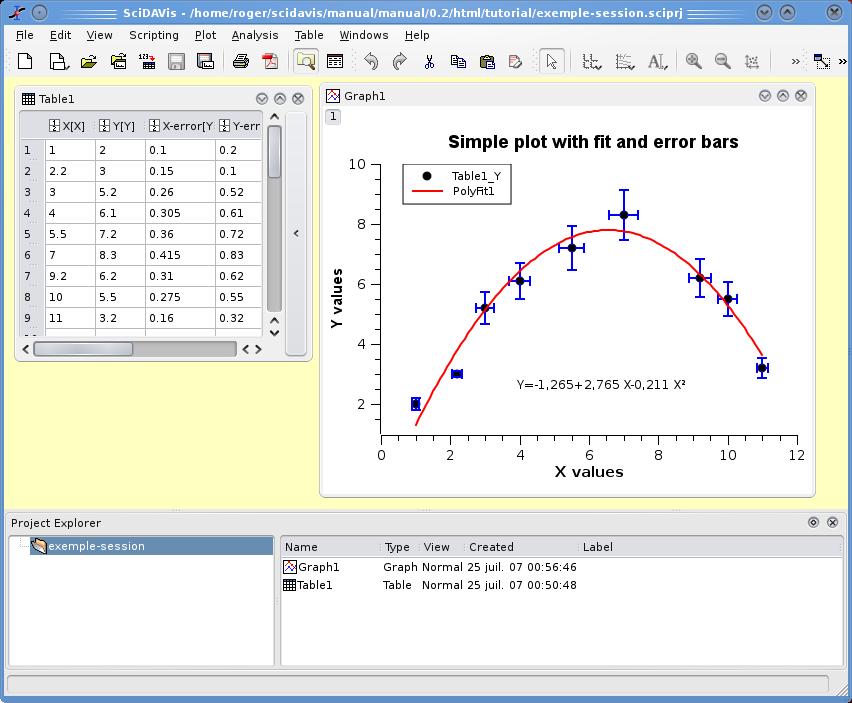
\includegraphics{pics/scidavis-session.png}}
  \caption{A typical \SciDaVis{} session}
  \label{fig-scidavis-session}
\end{figure}

There are numerous commands available in \SciDaVis{} depending on the
element which is selected. Therefore, the main menu bar changes when
you select a particular element of the project. Moreover, you can
access to the set of commands relevant of an element by activating the
context menu with the right button of the mouse.

In a project, the objects which can be used are:

\begin{description}
  \item[Tables]\index{Table}
    A table is a spreadsheet which can be used to store the datas you are entering. It can also be used to do some calculations and statistical analysis of datas. In each table, columns can be labelled as X-values or Y-values for 2D-plotting, or Z-values if you plan to build a 3D-plot. In addition, columns can be labelled as errors on X or on Y values (see \htmlref{Set Column as command}{set-column-as-lnk}).

    A table can be created by the \htmlref{New $\rightarrow$ New Table
      command}{new-table-lnk}. Then there are several ways to fill the
    table with your data. If you want to read a table from an ASCII
    file, you can import the data from the file to a table with the
    \htmlref{Import ASCII command}{import-ascii-lnk}. You can also
    enter each value from the keyboard, or copy and paste from another
    spreadsheet program. The last way to enter your data is to fill
    the table with the results of a mathematical function
    (\htmlref{Assign Formula command}{assign-formula-lnk} from the
    \htmlref{Table menu}{table-menu-lnk})
    
    \item[Matrix]\label{sec-intro-matrix}\index{Matrix} A matrix is a
      special table which is used to store the data points for surface
      3D plots. It contains Z-values and doesn't include any column or
      row which could be designated as X-values or
      Y-values. Nevertheless, you can specify the X-values and the
      Y-values with the \htmlref{Set Coordinates
        command}{set-coordinates-lnk} from the \htmlref{Matrix
        menu}{matrix-menu-lnk}.

      A matrix can be created by the \htmlref{New$\rightarrow$ New
        Matrix command}{new-matrix-lnk}. If you want to read a matrix
      from an ASCII file, you can import the data of the file to a
      table with the \htmlref{Import ASCII command}{import-ascii-lnk}
      and then convert this table to a matrix with the \htmlref{Conver
        to Matrix command}{convert-to-matrix-lnk}. In the same way as
      for tables, you can also fill matrix with the results of a
      function z=f(i,j) in which i and j are row and column numbers,
      or z=f(x,y). (see \htmlref{Assign Formula
        command}{assign-formula-lnk} from the \htmlref{Matrix
        menu}{matrix-menu-lnk})

    \item[A Graph]\label{sec-intro-plot-window}\index{Plot} A graph
      can contain one or several plots. Each of these plots is
      contained in a different {\em layer}, these layers can be
      arranged in many ways to build matrix of plots.

      A new layer can be added to an existing graph with the
      \htmlref{Add Layer command}{add-layer-lnk} from the
      \htmlref{Graph menu}{graph-menu-lnk}. you can also remove an
      existing layer with the \htmlref{Remove Layer
        command}{remove-layer-lnk}, but if you remove a layer, the
      plot will be deleted. You can also copy a layer from one graph
      to another, or copy an existing graph into another, the window
      will be added as a new layer (see the section on
      \htmlref{Multilayer Plots}{sec-multilayer-plots} for more
      details).

      Plots can be created in several ways. You can select data in
      tables or matrix and build a plot, or create new plots from
      functions of one or two variables (see sections \htmlref{2D
        plots}{sec-2d-plots} and \htmlref{3D plots}{sec-3d-plots}).

    \item[A Note]\label{sec-intro-note} This window is a text
      container which can simply be used to insert comments into a
      project. This object is nevertheless far more powerfull than
      that: it can be used as a calculator, for executing single
      commands and for writing scripts (see the \htmlref{Scripting
        section}{scripting} for more details).
      
    \item[The Log Window]\label{sec-intro-log-window}
      This window is used to store the results of all the calculations
      which have been done. If this window is not visible, you can
      find it with the \htmlref{Project
        Explorer}{sec-intro-project-explorer} or with the
      \htmlref{Result Log command}{results-log-lnk}.
      
      The text in the log window is also saved in the project file, so
      that when you load a previously saved project, the results-log
      panel is re-filled with the results of the calculations.

    \item[The Project Explorer]\label{sec-intro-project-explorer}
      This window is used to list all the windows contained in a
      project. The Project Explorer is opened by the \htmlref{Project
        Explorer command}{project-explorer-lnk}, and gives a quick
      access to all elements of a project, hidden or visibles. It can
      be used to do some operations on the windows related to these
      items such as hidding a window, renaming windows, etc.
      
      A project file can include several independant projects. In this case,
      the containers of each project are stored in different folders.

\end{description}
%		General description of a table
%		==============================

\subsection{Tables}\label{sec-intro-table}
\index{Table}

The table is the main part of \SciDaVis{} when working with data. For
controlling and converting data the spreadsheet contains a highly
customizable table: all colors and font preferences can be set using
the \htmlref{Preferences command}{preferences-lnk} of the \htmlref{Edit
  menu}{edit-menu-lnk}. You can resize a table
in terms of rows and columns using the \htmlref{Dimensions command}{table-dimensions-lnk} command
of the \htmlref{Table menu}{table-menu-lnk}. On the left side of the table, the button can
be used to develop the properties tags. This allows to customize the
main parameters of the table.

\begin{figure}
  \resizebox{\textwidth}{!}{
\includegraphics{pics/table.png}}
  \caption{A \SciDaVis{} table with the properties dialog developped
    and the type tag selected.}
  \label{fig-the-table}
\end{figure}

In a spreadsheet, columns can have the following flags: X, Y, Z,
X-error, Y-error or can be simple columns without any special
flag. The X columns are abscissae columns while the Y columns are
ordinates columns used when creating a 2D plot from data. The X-error
and Y-error columns can be used in order to add error bars to 2D
plots. These flags can be changed using the \htmlref{Set Column as
  command}{set-column-as-lnk}.

\index{Table!Number format}

The tag which is selected in figure \ref{fig-the-table} is used to
assign a type to columns: numeric, text, date or time. The format used
to display the data can then be chosen, the format in tables is not
used for plots (use the \htmlref{Axes command}{format-axes-lnk} to
define display format for axes labels).

\begin{figure}
  \resizebox{\textwidth}{!}{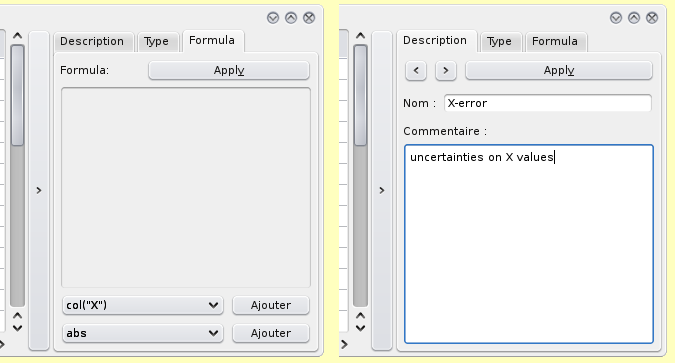
\includegraphics{pics/table_tag_1_3.png}}
  \caption{The two other tags of the properties dialog of \SciDaVis{} tables.}
  \label{fig-the-table_2}
\end{figure}

\index{Table!Labels}

Every column of the table has a label, this can be defined in the
description tag (figure \ref{fig-the-table_2}). This label will be
used by default in plots for curve selection and legend display. You
can use complex labels with spaces and special characters like ``Vol
(cc/g)" if needed. This command can also be reached by the
\htmlref{Edit Column Description command}{edit-column-description-lnk}
of the \htmlref{Table menu}{table-menu-lnk}.

\index{Table!Assign formula}

The last tag of the properties dialog correspond to the command
\htmlref{Assign Formula command}{assign-formula-lnk} of the
\htmlref{Table menu}{table-menu-lnk} (figure \ref{fig-the-table_2}). It is used to fill the column with the result of a mathematic expression. Refer to the \htmlref{Assign Formula command}{assign-formula-lnk} for more details.

You can select all the columns of the spreadsheet (\verb|Ctrl+A|) or
only some of them by clicking on the column label while keeping the
\verb+Ctrl+ key pressed, or by moving the mouse over the column
label. This also allows you to deselect columns.

On the selected columns you can perform various operations:

\begin{itemize}
\item Fill with data. You can insert the row numbers (\htmlref{Fill
  Selection With$\rightarrow$Row Numbers
  command}{fill-selection-with-row-number-lnk}), random numbers
  (\htmlref{Fill Selection With$\rightarrow$Random
  Values}{fill-selection-with-random-values-lnk}), or the result of a
  function (\htmlref{Assign Formula command}{assign-formula-lnk});
\item\index{table!normalize columns} normalize columns with the \verb+Normalize Columns+ command of the context menu;
\item\index{table!sort columns}  sort columns with the \htmlref{Sort
  Table command}{sort-table-lnk} of the \htmlref{Table
  menu}{table-menu-lnk} or with the \verb+sort column+ command of the
  context menu;
\item compute statistical data on columns and rows with the
  \htmlref{Statistics on Columns command}{statistics-on-columns-lnk}
  and \htmlref{Statistics on Rows command}{statistics-on-rows-lnk}
  of the \htmlref{Analysis-tables menu}{analysis-tables-menu-lnk};
\item build a plot from selected columns with the \verb+plot+ command
  of the context menu or with the commands of the \htmlref{Plot menu}{plot-menu-lnk}.
\end{itemize}

All these functions can be reached by right clicking when a column is
selected. Most of them can also be reached by using the \htmlref{Table
  menu}{table-menu-lnk}.

You can cut, copy and paste data between spreadsheets or between a
spreadsheet and another application (Excel, Gnumeric, OpenOffice Calc,
etc).
  
You can import single or multiple ASCII files using the
\htmlref{Import ASCII command}{import-ascii-lnk} from the
\htmlref{File menu}{file-menu-lnk}. This will create one or more new
tables. You can also export the data from the spreadsheet to a text
file using the \htmlref{Export ASCII command}{export-ascii-lnk}.

%</sect2>
%<!--
%		General description of a matrix
%		===============================
%-->
%<sect2 id="sec-intro-matrix">
%  <title>Matrix</title>
%  <indexterm><primary>Matrix</primary></indexterm>
%  <para>The matrix is a special table which is used for data which depends on two variables. This special table is used to store data for 3D-plots. The difference between a table and a matrix is that there is that columns are assigned to the abscissae x while rows define abscissae y.</para>
%  <para>The defaut size of a matrix is 32x32 cells. You can modify this size with the &matrix-dimensions-lnk;. Column and row numbers are named i and j respectively, ranging from 1 to the size of the matrix. You can specify an X-scale and an Y-scale with the &set-coordinates-lnk;, this define values of x and y for columns and rows (figure <xref xrefstyle="select: labelnumber" linkend="fig-matrix"/>).</para>
%
%<figure id="fig-matrix">
%  <title>The &appname; matrix</title>
%  <mediaobject>
%    <imageobject>
%      <imagedata  format="PNG" fileref="pics/matrix.png"/>
%    </imageobject>
%  </mediaobject>
%</figure>
%
%  <para>The values which are stored in a matrix can be obtained from a function of the form z=f(i,j) or z=f(x,y) with the &assign-formula-lnk;. They can also be read from a file with the &import-ascii-lnk; which allows to read a file in a table, then the table can be converted to a matrix with the &convert-to-matrix-lnk; of the &matrix-menu-lnk;.</para>
%  <para>As in the case of tables, a property tag can be shown or hidden by clicking on the vertical button on the right.</para>
%  <para>Through the &matrix-menu-lnk;, several operations can be done on a matrix like transposition (&transpose-lnk;), mirroring (&mirror-horizontally-lnk; and &mirror-vertically-lnk;), inversion (&invert-lnk;), computation of the determinant (&determinant-lnk;). The data of a matrix can then be used to build a 3D plot with the commands present in the &plot3d-menu-lnk; and in &d3-surface-toolbar-lnk;.</para>
%
%</sect2>
%
%<!--
%		General description of a plot window
%		====================================
%-->
%<sect2 id="sec-intro-plot-window">
%<title>Plot Window</title>
%
%<indexterm><primary>Plot</primary></indexterm>
%<indexterm><primary>Plot</primary><secondary>Layer</secondary></indexterm>
%
%<para>The plot window is the one in which the graphic is plotted. The main container of the plot window is the layer. You can have several layers in a plot, which may be arranged as you want. Each layer can contain a plot, or another item like a label.</para>
%<para>Each new plot can be inserted in a new layer of this plot window, it has its own geometry and graphic properties (background color, frame, etc). The figure <xref xrefstyle="select: labelnumber" linkend="fig-plot-window"/> shows a graph with two layers which have different geometries. Inside a layer, the area in which the curves are plotted is the <emphasis>canvas</emphasis>.</para>
%
%<figure id="fig-plot-window">
%  <title>An example of &appname; 2D graph with 2 layers.</title>
%  <mediaobject>
%    <imageobject>
%      <imagedata  format="PNG" fileref="pics/plot-window.png"/>
%    </imageobject>
%  </mediaobject>
%</figure>
%
%<para>Each layer can be activated by clicking on the corresponding gray button  <inlinemediaobject><imageobject><imagedata format="PNG" fileref="pics/layer-button.png"/></imageobject></inlinemediaobject> in the top-left corner of the window. The elements which can be accessed by a double click in a layer are:</para>
%
%<itemizedlist>
%<listitem>
%<para>the graph itself: this will open the <link linkend="
%format-plot-cmd">Plot details</link> dialog box. You can then change the way the curves are plotted.</para>
%</listitem>
%<listitem>
%<para>The axes or the axes labels: this will open the <link linkend="format-axes-cmd">General Plot Options Dialog</link>. It is used to customize the axes, the numbers and labels of the axes, and the grid.</para>
%</listitem>
%<listitem>
%<para>Any other text item: this will open the <link linkend="sec-adding-text">Text Dialog</link> which allows to customize the font of the label and the frame in which it is drawn.</para>
%</listitem>
%</itemizedlist>
%
%<para>All these functions can be reached through the &format-menu-lnk;.</para>
%</sect2>
%
%<!--
%		General description of a note
%		=============================
%-->
%<sect2 id="sec-intro-note">
%<title>Note</title>
%
%<indexterm><primary>Note</primary></indexterm>
%<para>A note can simply be used to insert text (comments, notes, etc) into a project, but is really far more powerfull than that. It can be used as a calculator, for executing single commands and for writing scripts.</para>
%
%<figure id="fig-note-window">
%  <title>The &appname; Note Window</title>
%  <mediaobject>
%    <imageobject>
%      <imagedata  format="PNG" fileref="pics/new-note1.png"/>
%    </imageobject>
%  </mediaobject>
%</figure>
%
%<para>You can also change the text input method. <emphasis>Simple Composing Input Method</emphasis> is the standard method to enter text in QT applications. <emphasis>Xim</emphasis> is the X input method, it is the legacy system of the X window environment to support localized text input. The default choice is the second one, it allows to enter special characters and accents from your localised environment.</para>
%
%<indexterm>
%  <primary>Calculator</primary><see>Note</see>
%</indexterm>
%
%<para>The second use of notes is calculator. The evaluation of mathematical expressions and execution of code is done via a note's context menu, the Scripting menu or the convenient keyboard shortcuts. In figure <xref xrefstyle="select: labelnumber" linkend="fig-note-window-1"/>, it is shown that you just need to place the cursor on an expression and use the <keycode>Ctrl-Return</keycode> command to evaluate the expression.</para>
%
%<figure id="fig-note-window-1">
%  <title>The &appname; Note Window used as a calculator</title>
%  <mediaobject>
%    <imageobject>
%      <imagedata  format="PNG" fileref="pics/new-note2.png"/>
%    </imageobject>
%  </mediaobject>
%</figure>
%
%<para>you can define variables and refer to them to build complex expressions, but you must evaluate each line with the <keycode>Ctrl-Return</keycode> command to fill the variable with its value. All variable are private to the note in which it is defined, and you can't refer to it in another note. With a right click, you access to the context menu which contains the list of all available mathematical functions.</para>
%
%<para>For information on expression syntax, supported mathematical functions and how to write scripts, see the <link linkend="scripting">scripting section</link>.</para>
%
%</sect2>
%
%<!--
%		General description of the log window
%		=====================================
%-->
%<sect2 id="sec-intro-log-window">
%<title>Log Window</title>
%<indexterm>
%  <primary>Log Window</primary>
%</indexterm>
%<indexterm>
%  <primary>Analysis</primary><secondary>Results</secondary>
%</indexterm>
%
%<para>This window keeps a history of all analysis which have been done in the project. This panel contains the results of all the correlations, fittings, etc. It can be shown or hidden with the &results-log-lnk; of the &view-menu-lnk;.</para>
%
%<figure id="fig-log-window">
%  <title>The &appname; Log window with the information related to a fit on a curve</title>
%  <mediaobject>
%    <imageobject>
%      <imagedata  format="PNG" fileref="pics/log-window.png"/>
%    </imageobject>
%  </mediaobject>
%</figure>
%<para>You can clear the content of the log window with the command &clear-log-information-lnk; of the &edit-menu-lnk;. If you load a project for which some analysis has been done, the computations will be done again and the log window will be filled with the results.</para>
%
%</sect2>
%
%<!--
%		General description of the project explorer
%		===========================================
%-->
%<sect2 id="sec-intro-project-explorer">
%<title>The Project Explorer</title>
%<indexterm>
%  <primary>Project Explorer</primary>
%</indexterm>
%
%<para>The project explorer can be opened/closed using the &project-explorer-lnk; from the &view-menu-lnk; or by clicking on the &project-explorer-icon; in the <link linkend="sec-file-toolbar">file toolbar</link>.</para>
%
%<figure id="fig-project-explorer">
%  <title>The &appname; Project Explorer</title>
%  <mediaobject>
%    <imageobject>
%      <imagedata  format="PNG" fileref="pics/explorer1.png"/>
%    </imageobject>
%  </mediaobject>
%</figure>
%
%<para>It gives an overview of the structure of a project and allows the user to perform various operations on the windows (tables and plots) in the workspace: hiding, minimazing, closing, renaming, printing, etc... These functions can be reached via the context menu, by right-clicking on an item in the explorer.</para>
%<para>By double-clicking on an item, the corresponding window is shown maximized in the workspace, even if it was hidden before.</para>
%<para>You can organize the differents objects in folders. When selecting a folder, the default policy is that only the objects contained in it will be showed in the workspace window. You can also display all the objects in the subfolders if you change this policy with the "View Windows" command to "Windows in Active Folder and Subfolders".</para>
%
%</sect2>
%
%</sect1>


